\documentclass[tikz,border=0pt]{standalone}
\usepackage[american]{circuitikz}
\usetikzlibrary{arrows.meta,calc,positioning,decorations.pathmorphing,patterns}
\definecolor{zyloTeal}{HTML}{174A5B}
\definecolor{zyloTealTwo}{HTML}{246B7A}
\definecolor{zyloInk}{HTML}{1F2933}
\definecolor{zyloSoft}{HTML}{EAF4F4}
\definecolor{zyloPaper}{HTML}{F8FAFB}
\definecolor{zyloLine}{HTML}{44606B}
\definecolor{zyloOrange}{HTML}{D97706}
\begin{document}
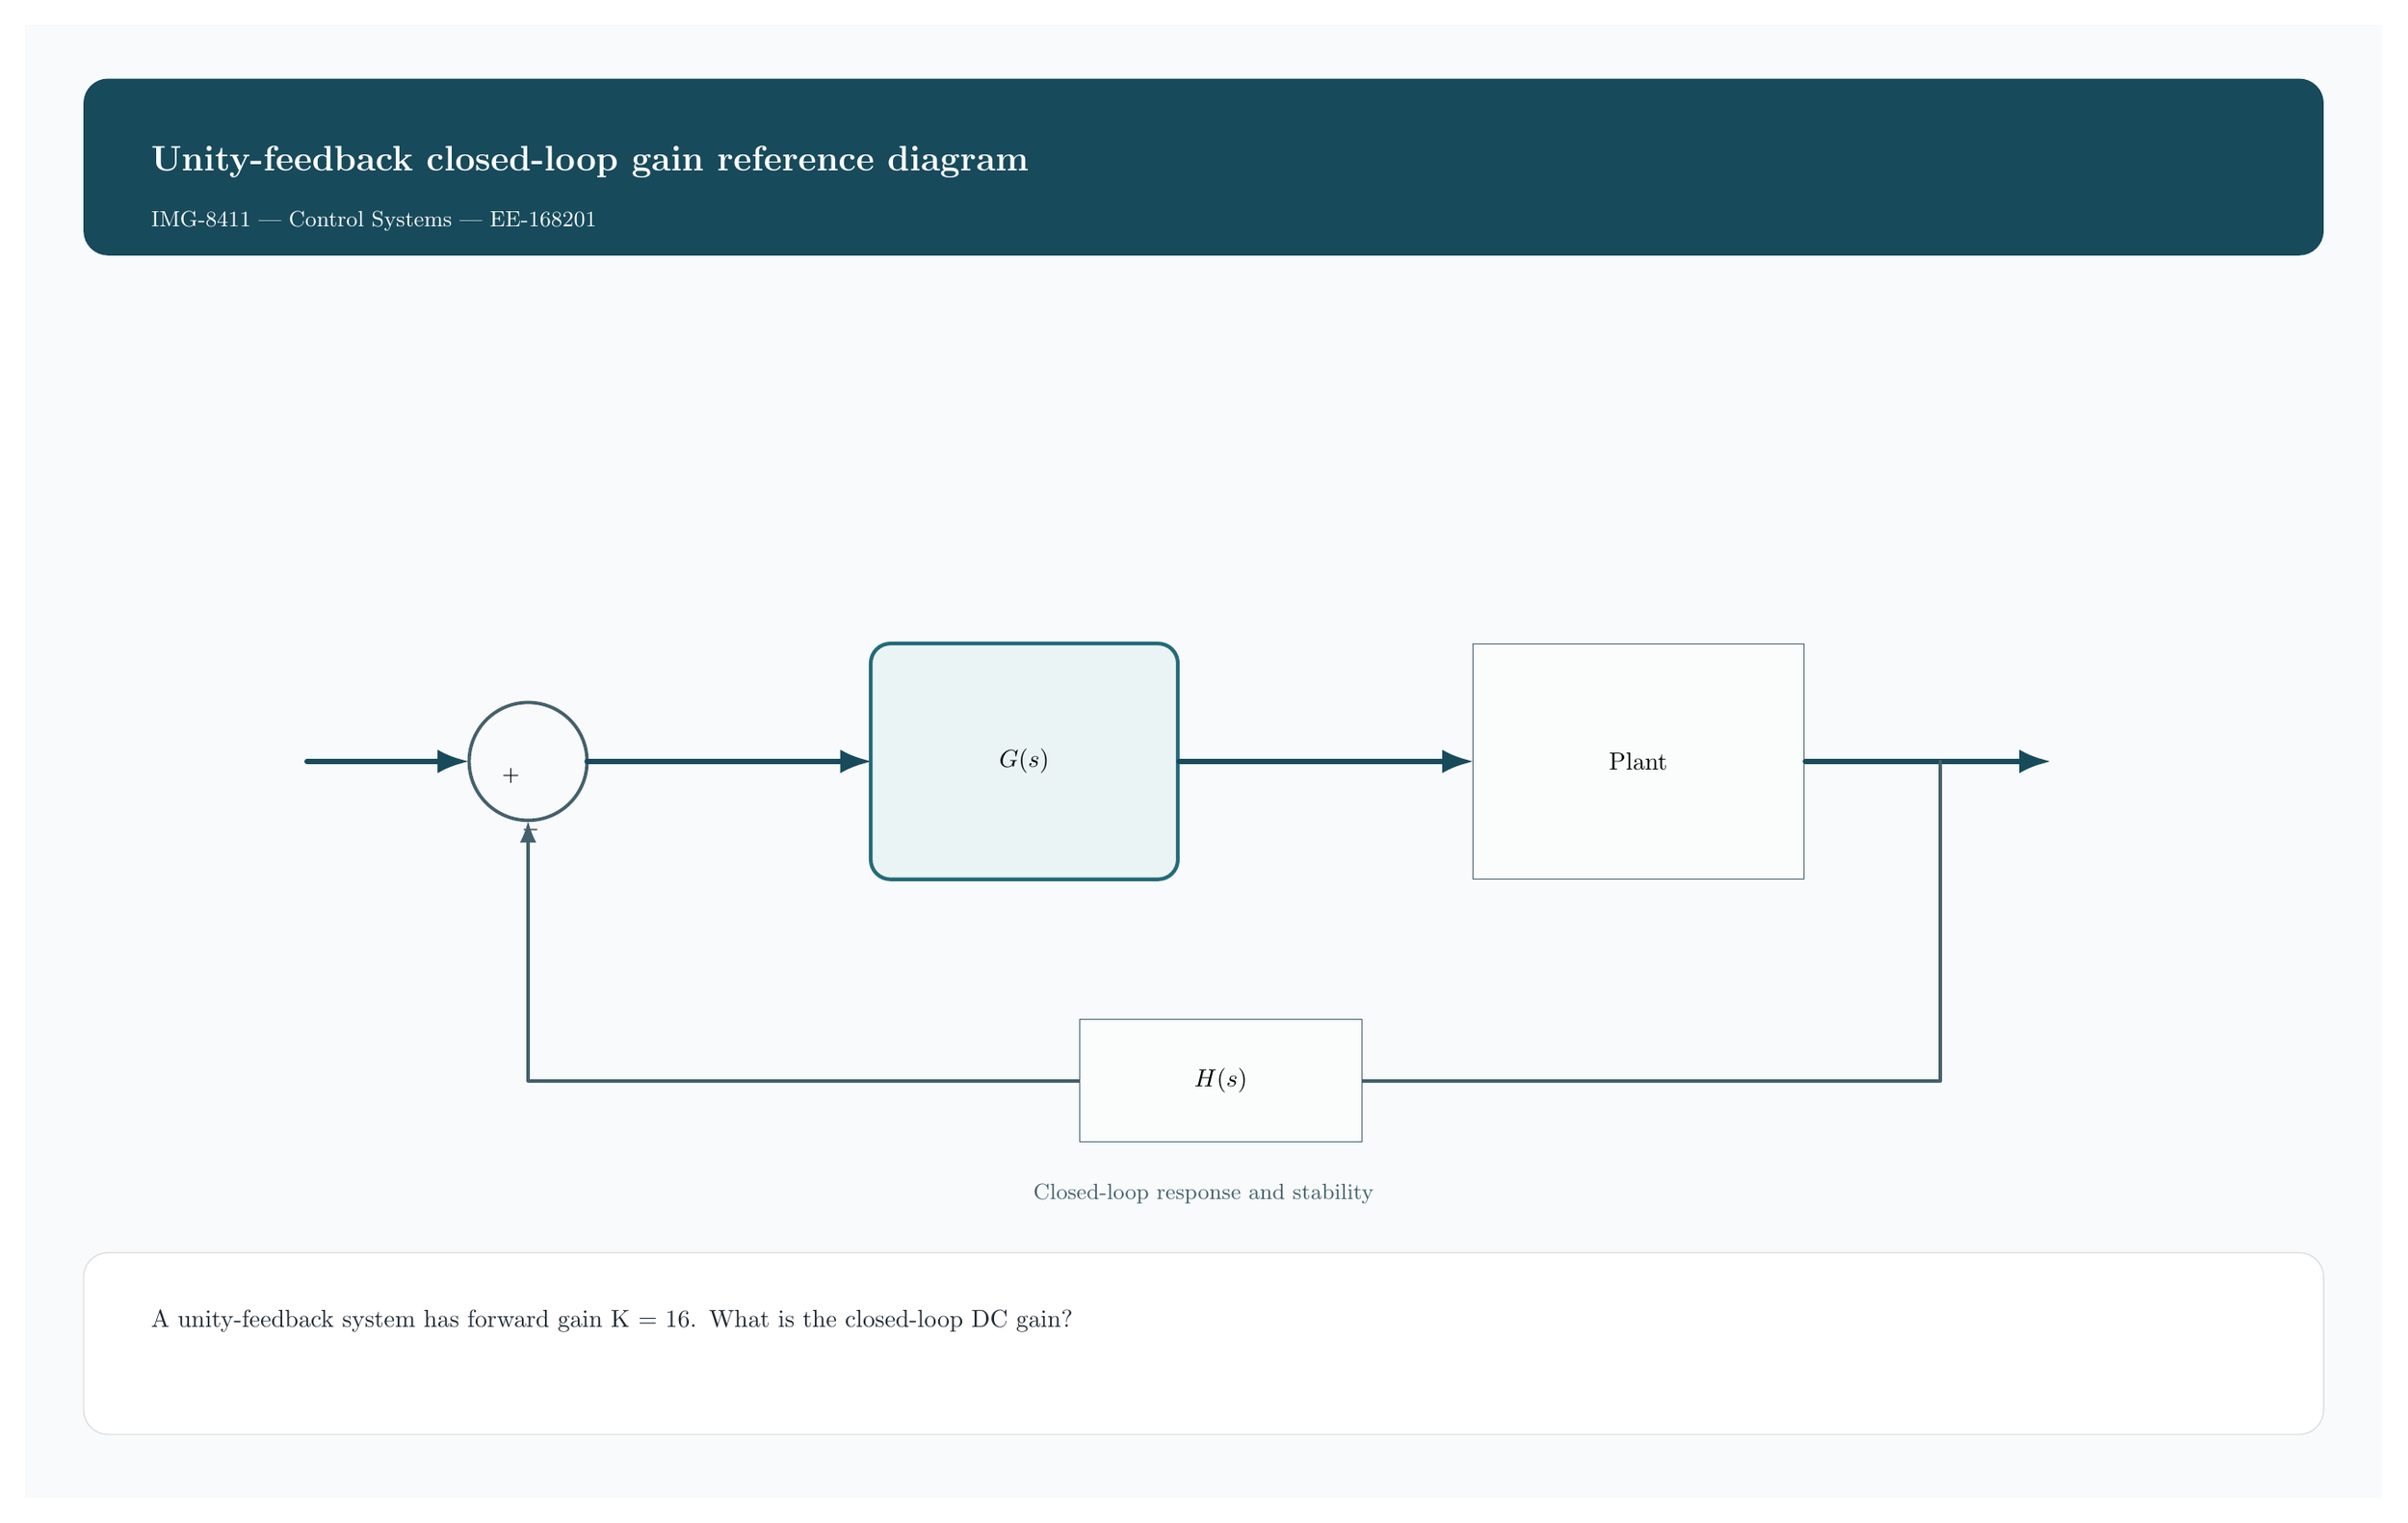
\begin{tikzpicture}[x=1pt,y=-1pt,>=Latex,line cap=round,line join=round]
\path[fill=zyloPaper] (0,0) rectangle (960,600);
\path[fill=zyloTeal,rounded corners=10pt] (24,22) rectangle (936,94);
\node[anchor=west,text=white,font=\bfseries\Large] at (48,56) {Unity-feedback closed-loop gain reference diagram};
\node[anchor=west,text=white!82,font=\small] at (48,80) {IMG-8411 | Control Systems | EE-168201};
\tikzset{wire/.style={draw=zyloTeal,line width=2.2pt},thinwire/.style={draw=zyloLine,line width=1.35pt},accent/.style={draw=zyloOrange,line width=2.2pt},box/.style={draw=zyloTealTwo,fill=zyloSoft,line width=1.5pt,rounded corners=8pt}}
\draw[thinwire] (205,300) circle (24); \node[font=\small] at (198,306) {$+$}; \node[font=\small] at (206,328) {$-$};
\draw[wire,->] (115,300) -- (181,300); \draw[wire,->] (229,300) -- (345,300);
\node[box,minimum width=125pt,minimum height=96pt] at (407,300) {$G(s)$};
\draw[wire,->] (470,300) -- (590,300);
\node[draw=zyloLine,fill=white!80!zyloSoft,minimum width=135pt,minimum height=96pt] at (657,300) {Plant};
\draw[wire,->] (725,300) -- (825,300);
\draw[thinwire,->] (780,300) -- (780,430) -- (205,430) -- (205,324);
\node[draw=zyloLine,fill=white!80!zyloSoft,minimum width=115pt,minimum height=50pt] at (487,430) {$H(s)$};
\node[font=\small,text=zyloLine] at (480,476) {Closed-loop response and stability};
\path[draw=black!15,fill=white,rounded corners=10pt] (24,500) rectangle (936,574);
\node[anchor=west,text width=860pt,align=left,text=zyloInk,font=\normalsize] at (48,528) {A unity-feedback system has forward gain K = 16. What is the closed-loop DC gain?};
\end{tikzpicture}
\end{document}
